\chapter{Introduction to LLM}

\section{What is a Language Model (LM)?}

A Language Model is a probabilistic model of a natural language. It produce a probability for any sequence of words.

The probability over all possible sentences in a language sums to 1.
There are region of high density in the space of all possible sentences.

\subsection{Formal definition for language models}

\begin{equation*}
  P(w1, w2, ..., wn) = \prod_{t=1}^{T} P(w_t | w_1, w_2, ..., w_{t-1})
\end{equation*}


\section{Simple LMs - n-gram models}

We need to estimate the probability of a word given the previous words.
A simplifying assumption, Markov assumption, is that:

\begin{equation*}
  P(w_t | w_1, w_2, ..., w_{t-1}) \approx P(w_t | w_{t-n+1}, ..., w_{t-1})
\end{equation*}

The next word $w_t$ depends only on a small windows of $n-1$ preceding words called the \textbf{context}.


For $n=2$, the next word only depends on the previous word, called a \textbf{bigram} model.
\begin{equation*}
  P(w_t | w_{t-1}, w_{t-2}, ..., w_1) \approx P(w_t | w_{t-1})
\end{equation*}


\section{Estimation \& generation}

We can use a language model to estimate probabilities for new
sentences.
Generate a new sentence based on known probabilities.

\begin{itemize}
  \item Starting from a given word, we can compute the probability of having any
        other word following it
  \item Then, we choose one word based on this probability distribution
  \item We add the new word to the already available sequence, and generate the
        next one
  \item We call this, autoregressive generation
\end{itemize}


\paragraph{Example}

$P(the, cat, chased, the, cheese) = P(the) \times P(cat | the) \times P(chased | the, cat) \times P(the | the, cat, chased) \times P(cheese | the, cat, chased, the)$

We can use the Markov assumption to simplify the computation of the probabilities.

$P(the, cat, chased, the, cheese) \approx P(the) \times P(cat | the) \times P(chased | cat) \times P(the | chased) \times P(cheese | the)$

Let's assume $P(the) = 1$

$P(the, cat, chased, the, cheese) \approx 1 \times \frac{1}{4} \times 1 \times 1 \times \frac{1}{4} = \frac{1}{16}$


\section{Generating new sentences}



\section{Limitation of n-grams}

\begin{enumerate}
  \item \textbf{Data sparsity}: As n increases, the number of possible n-grams grows exponentially. Bigram, V words, the table size is $V^2$. n-grams, V words, the table size is $V^n$. A small vocabulary or a small context size make the LM quite useless
  \item \textbf{Context limitation}: Only local context (previous n-1 words) are used to choose. Longer sentences may require remembering what happened "early on"
  \item \textbf{Lack of semantics}:Similar words are treated in the same way as completely different ones
\end{enumerate}

The languafe models are not a new concept. In the '90s, researchers tried to build LMs based on existing
techniques and computing capabilities. With varying results... Mostly bad.


\section{Bigger and better Language Models}



We can see $P(w_t | w_{t-1}, w_{t-2}, ..., w_1)$ as a classification function.

"Given an \textbf{input}, the previous words in the sentence, predict the \textbf{next word}, class."



\chapter{Introduction to deep learning}

\section{The perceptron}


\begin{flushleft}
  \begin{minipage}{0.65\linewidth}

    The perceptron is the simplest unit of \textbf{neural networks}. It takes an input with multiple features and \textbf{multiplies} it by
    a weight. Then, it sums all the weighted inputs and applies a non-linear function to produce an output.

    \begin{equation*}
      y = f(w_0 + w_1x_1 + w_2x_2 + ... + w_nx_n)
    \end{equation*}

    Where:

    \begin{itemize}
      \item $y$ is the output of the perceptron
      \item $f$ represents a non-linear "activation" function
      \item $w_i$ and $w_0$ are the weights and bias witch are learned during training
      \item $x = (x_1, x_2, ..., x_n)$ are the inputs to the perceptron
    \end{itemize}


  \end{minipage}%
  \hfill
  \begin{minipage}{0.3\linewidth}
    \centering
    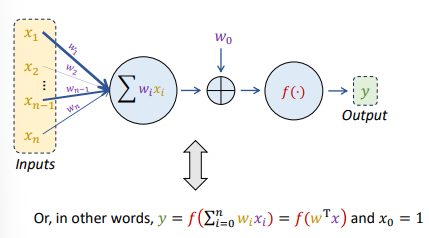
\includegraphics[width=1\linewidth]{content/Parts/images/2026-09-21-09-33-07.png}
  \end{minipage}
\end{flushleft}




\section{The perceptron, in 2D}

\begin{center}
  \begin{minipage}{0.65\linewidth}
    If the $f$ function is a linear activation function $f(x) = x$ then the equation is $y = w_1x_1 + w_2x_2 + w_0$.

    Various values of $w_0$, $w_1$, $w_2$ defie the different functions that can be learned by the perceptron.

    In this way perceptron can be used to represent a family of functions.

  \end{minipage}%
  \hfill
  \begin{minipage}{0.3\linewidth}
    \centering
    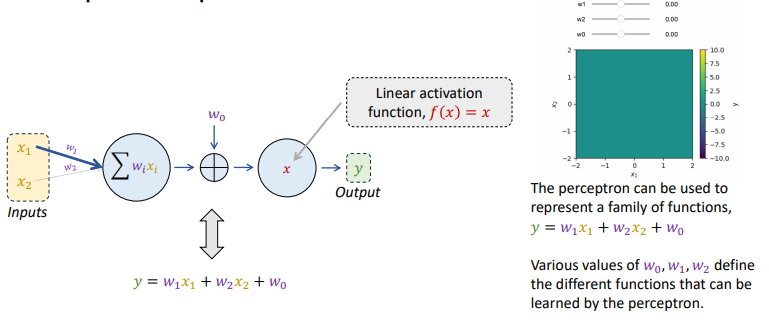
\includegraphics[width=1\linewidth]{content/Parts/images/2026-09-21-09-36-40.png}
  \end{minipage}
\end{center}


\section{Activation functions}


\begin{flushleft}
  \begin{minipage}{0.65\linewidth}
    Activation functions are used for two main reasons:

    \begin{enumerate}
      \item Enforce properties on perceptron's output. E.g. sigmoid $\to$ binds output to [0, 1] range
      \item Introduce non-linearities in the model + some others (faster convergence, sparsity, ...)
    \end{enumerate}


    Common activation functions are: ReLU, Sigmoid, Leaky ReLU, Tanh, Softmax, Linear, GeLU

  \end{minipage}%
  \hfill
  \begin{minipage}{0.3\linewidth}
    \centering
    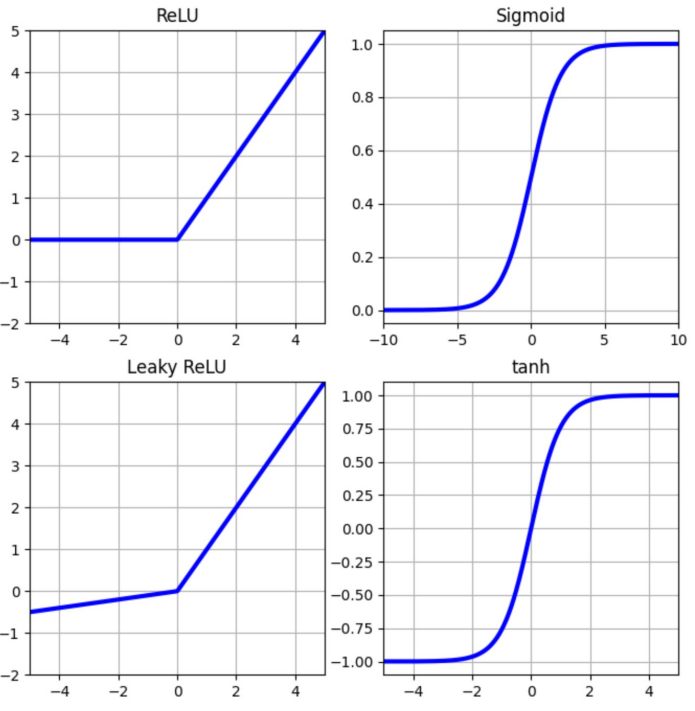
\includegraphics[width=1\linewidth]{content/Parts/images/2026-09-21-09-41-37.png}
  \end{minipage}
\end{flushleft}


\subsection{Enforce properties on perceptron's output}


\begin{center}
  \begin{minipage}{0.65\linewidth}
    Binary classification problem: seprate positive ($\star$) and negative ($\circ$) samples. For a point $x \in \Re^2$,
    the perceptron can predict $p(\star | x)$. For a binary case this implies that $p(\circ | x) = 1 - p(\star | x)$.

    To get a valid probability, we must enforce $p(\star | x) \in [0, 1]$.
    We already have $p(\circ | x ) + p(\star | x) = 1 $ by construction

    The Sigmoid maps any value in $\Re$ to the range $[0, 1]$. The output is squashed between 0 and 1.

    \begin{equation*}
      \sigma(x) = \frac{1}{1 + e^{-x}}
    \end{equation*}

  \end{minipage}%
  \hfill
  \begin{minipage}{0.3\linewidth}
    \centering
    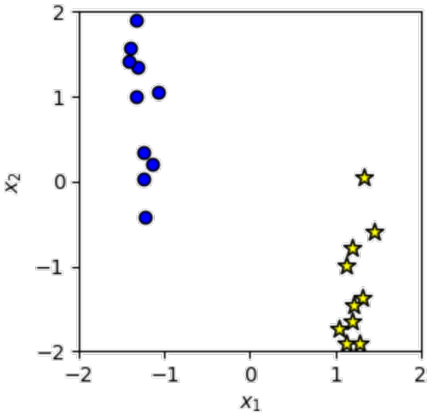
\includegraphics[width=1\linewidth]{content/Parts/images/2026-10-18-15-41-35.png}
  \end{minipage}
\end{center}

\subsection{Adding some perceptrons and adding other layers!}


\begin{center}
  \begin{minipage}{0.47\linewidth}
    \centering
    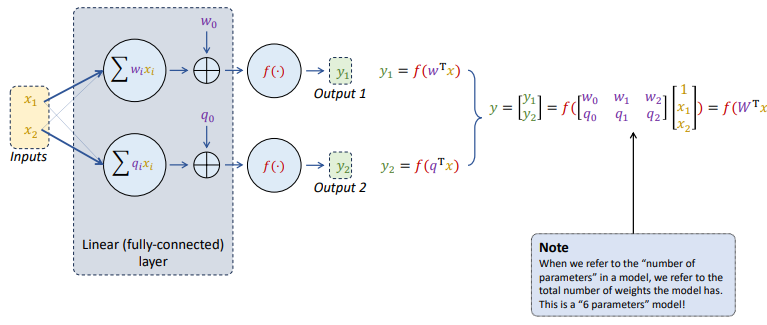
\includegraphics[width=1\linewidth]{content/Parts/images/2026-09-21-09-50-18.png}
  \end{minipage}%
  \hfill
  \begin{minipage}{0.47\linewidth}
    \centering
    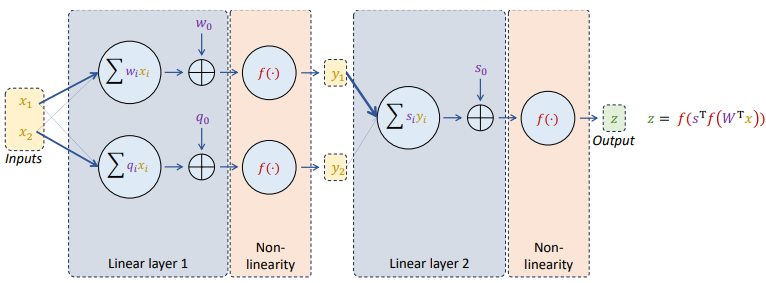
\includegraphics[width=1\linewidth]{content/Parts/images/2026-09-21-09-51-10.png}
  \end{minipage}
\end{center}


\subsection{Introduce non-linearities in the model}




\begin{flushleft}
  \begin{minipage}{0.75\linewidth}


    This is the second reason why we need activation functions.

    If $f(x) = x$ (i.e., no non-linearity is added) we get $z = s^T W^T x$


    This implies:
    \begin{enumerate}
      \item We could have used $W' = W_s$ and get the same output
      \item We wouldn't have needed a second layer!
      \item But our model is still linear
    \end{enumerate}

    So, we use non-linear activation functions to
    model more complex functions
  \end{minipage}%
  \hfill
  \begin{minipage}{0.2\linewidth}
    \centering
    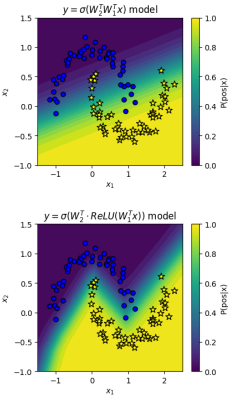
\includegraphics[width=0.7\linewidth]{content/Parts/images/2026-10-18-15-48-23.png}
  \end{minipage}
\end{flushleft}


\section{Multi-layer perceptron models}

\begin{flushleft}
  \begin{minipage}{0.65\linewidth}

    We can stack additional layers separated by non-linearities (activation functions) to prevent collapses.

    Universal Approximation Theorem tells us that
    we can approximate "any" function with MLPs.

    "For any continuous function $g$ defined on a compact
    subset of $\Re^n$ and for any $\epsilon > 0$, there exists a
    feedforward neural network with a single hidden
    layer and a finite number of neurons that can
    approximate g to within an arbitrary degree of
    accuracy $\epsilon$"

    A single-layer MLP works … but no information on the
    number of neurons, or the weights' values!
    Deeper, narrower networks are generally used

  \end{minipage}%
  \hfill
  \begin{minipage}{0.3\linewidth}
    \centering
    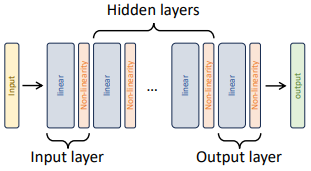
\includegraphics[width=1\linewidth]{content/Parts/images/2026-10-18-16-07-49.png}
  \end{minipage}
\end{flushleft}


\section{Activation functions for classification models}


\begin{flushleft}
  \begin{minipage}{0.65\linewidth}
    As argued, activation functions can be used to enforce properties on
    the model's output

    In classification problems, the output before the final activation is
    treated as unnormalized probabilities \textbf{logits unit}.

    We still need a step to convert logits into valid probabilities. E.g. all probabilities must sum to 1 and be in the range [0, 1].

  \end{minipage}%
  \hfill
  \begin{minipage}{0.3\linewidth}
    \centering
    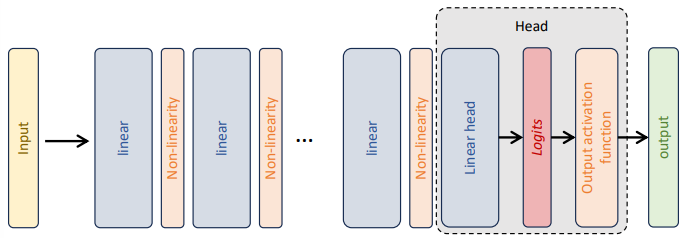
\includegraphics[width=1\linewidth]{content/Parts/images/2026-09-21-10-18-55.png}
  \end{minipage}
\end{flushleft}


\section{Binary classification}

\begin{flushleft}
  \begin{minipage}{0.65\linewidth}

    The model predicts the probability of a single class for point $x$.
    As a convention, the positive one $P(pos|x)$.

    The model produces a logit $z = model(x)$. We use the \textbf{Sigmoid function} on the output logit z: $\sigma(z) = \frac{1}{1 + e^{-z}}$. This guarantees $P(pos|x)$ is in the range [0, 1].

    We work out the probability of the negative class $P(neg|x) = 1 - P(pos|x)$. We can easily show that $P(neg|x) \in [0, 1]$.

    By construction, $P(pos|x) + P(neg|x) = 1$.

  \end{minipage}%
  \hfill
  \begin{minipage}{0.3\linewidth}
    \centering
    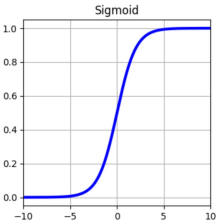
\includegraphics[width=0.65\linewidth]{content/Parts/images/2026-10-18-16-22-59.png}
  \end{minipage}
\end{flushleft}



\section{Multi-class classification}



\begin{flushleft}
  \begin{minipage}{0.65\linewidth}
    The output class is one of many classes ($c_1$, $c_2$, ..., $c_n$).
    The model produces n logit for a point $x$. I.e. the last layer have n perceptrons. $z = (z_1, z_2, ..., z_n) = model(x)$

    We need to obtain, from the logits, valid probabilities.
    $P(c_1|x)$, $P(c_2|x)$, ..., $P(c_n|x)$.

    The \textbf{softmax} function produce a probability of class (e.g. class 1 (cat), class 2 (dog)), it gives us
    only values between 0 and 1

    \begin{equation*}
      P(c_i|x) = \frac{e^{z_i}}{\sum_{j} e^{z_j}}
    \end{equation*}

  \end{minipage}%
  \hfill
  \begin{minipage}{0.3\linewidth}
    \centering
    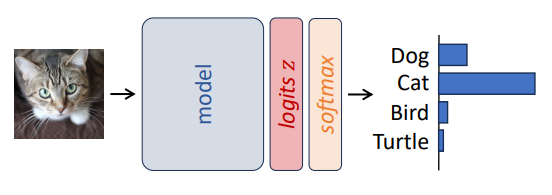
\includegraphics[width=1\linewidth]{content/Parts/images/2026-09-21-10-28-21.png}
  \end{minipage}
\end{flushleft}


\section{Activation functions for regression models}
In regression, models generally predict real numbers.
Typically, there is no need to enforce properties.
Output activation function can be the identity function $f(x) = x$.
Generally the only situation where it makes sense to use it!



\section{Defining weights (parameters)}

So far, we assumed all weights and biases (let's call them $\theta$) to be
known. But, we still need to figure out how we find them!

We pick a function, onjective or loss, $\mathcal{L}(\theta)$, that we want to minimize.

in Linear Regression we minimize the Mean Squared Error

It looks at the model, the data are fixed, and give us a number, high number means bad model, low number means good model.

\paragraph{Example:} $$\mathcal{L}(\theta) = MSE(\theta) = \frac{1}{n}\sum (y_i - \theta^T x_i)^2$$

Then, we pick $\theta$ that minimizes it

\begin{tcolorbox}
  \textbf{Note:} $\mathcal{L}$ also depends on the training points $x_i$, $y_i$, so we should
  refer to it as $\mathcal{L}(\theta, X, y)$.
  However, the training set $X$, $y$ is generally fixed. Thus, we
  only have control over $\theta$, so we use the notation $\mathcal{L}(\theta)$.
\end{tcolorbox}


\section{Linear regression}


\begin{flushleft}
  \begin{minipage}{0.65\linewidth}

    For simple models, we can find the optimal weights in closed form

    \begin{equation*}
      \frac{\partial \mathcal{L}(\theta)}{\partial \theta} = \frac{\partial MSE(\Theta)}{\partial \theta} = 0
    \end{equation*}

    $\\$Quadratic in $\theta$, can be solved easily!

      Or, we can evaluate the loss function for a bunch of $\theta$'s, and find the
      "best" one

      \begin{tcolorbox}
      \textbf{Note:} For linear regression, we don't try a bunch of $\theta$'s,
    since we can easily find the best value in closed
    form.
    However, this provides the intuition for what we
    will do next with more complex loss
    functions/models.
    \end{tcolorbox}

  \end{minipage}%
  \hfill
  \begin{minipage}{0.3\linewidth}
    \centering
    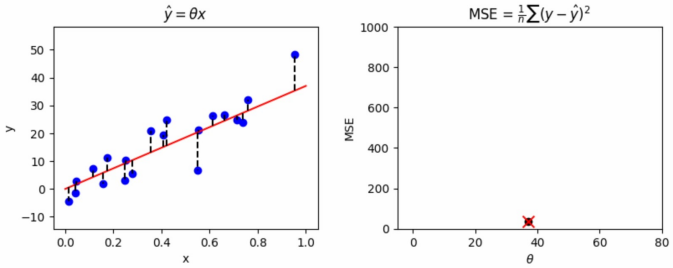
\includegraphics[width=1\linewidth]{content/Parts/images/2026-10-18-17-04-10.png}
  \end{minipage}
\end{flushleft}


\section{More complex losses/model}


\begin{flushleft}
  \begin{minipage}{0.65\linewidth}

    In more complex loss functions/models, we may not be able to solve the problem in a closed form.
    But we can evaluate $\mathcal{L}(\theta)$  for various values of $\theta$.


    We can iteratively update $\theta$ to reach a local minimum. We can start from a random value $\theta$, then "move around" according to "some policy"


    \textbf{Move around} = update $\theta$ incrementally, based on its current value. The new value of $\theta$
    at any step depends on the previous step's value: $\theta_{t+1} := \theta_t + \textit{update}$


    \textbf{Some policy} = we take a small step in the direction where the
    function decreases locally. i.e. in the \textbf{opposite} direction of the \textbf{gradient}.$\\$
    $\theta_{t+1} := \theta_t - \alpha \nabla_\theta \mathcal{L}(\theta_t)$

  \end{minipage}%
  \hfill
  \begin{minipage}{0.3\linewidth}
    \centering
    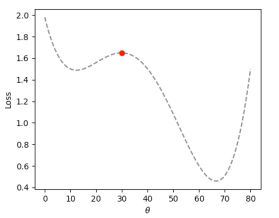
\includegraphics[width=1\linewidth]{content/Parts/images/2026-10-18-17-07-56.png}
  \end{minipage}
\end{flushleft}

For 1-dimensional $\theta$, we have $\theta_{t+1} := \theta_t - \alpha \frac{\partial \mathcal{L}(\theta)}{\partial \theta}$


Where $\alpha$: learning rate, controls the "size" of the step ($10^{-3}$, $10^{-4}$, etc)

This is called \textbf{gradient descent} (GD). We can visualize it as "going down the hill" of the loss function.

If the derivative is negative, I  move to the right, when the derivative is positive I  move to the left and
I get the bottom of the function.

Gradient Descent!

\subsection{Limitation of gradient descent}

GD is sensitive to weight initialization. Different initializations can lead to different solutions!
GD can get stuck in local minima


Various solutions to help prevent local minima:
\begin{itemize}
  \item Adding momentum
  \item Adaptive learning rates, how to regulate the step
  \item Learning rate schedules
\end{itemize}

\section{Backpropagation}

How to compute the gradient of a loss function with respect to the weights of a neural network?

So far, we assumed we were able to compute $\nabla_\theta \mathcal{L}(\theta)$.

We need some automated way to compute gradients.

Now we introduce the \textbf{backpropagation}, to compute the gradient of the loss w.r.t.
any weight! Backpropagation is just a fancy word for "using the chain rule"

\subsection{Using the chain rule}

We use the chain rule from calculus

\begin{equation*}
  \frac{\partial f}{\partial x} = \frac{\partial f}{\partial g} \frac{\partial g}{\partial x}
\end{equation*}

$\\$Other notation caould be $f(g(x))' = f'(g(x)) \cdot g'(x)$

  And apply it from the end of the computational graph, backwards. Hence the name, backpropagation.


  \subsection{Computational graph}


  \begin{flushleft}
  \begin{minipage}{0.65\linewidth}

  A computational graph is a directed graph
  \begin{itemize}
    \item Each node corresponds to an operation
    \item Each edge represents the flow of data between nodes
  \end{itemize}

  For instance, we may want to compute $y = wx + b$
  \end{minipage}%
  \hfill
  \begin{minipage}{0.3\linewidth}
    \centering
    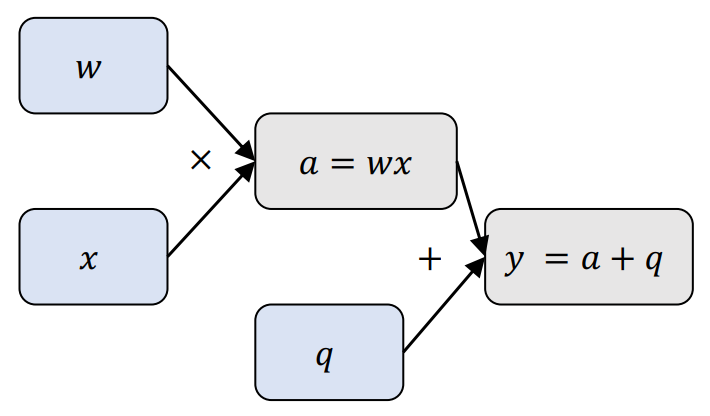
\includegraphics[width=1\linewidth]{content/Parts/images/2026-09-21-11-02-42.png}
  \end{minipage}
  \end{flushleft}


  We start from three variables, $w$, $x$ and $y$. The computational graph performs one
  operation at a time.


  \begin{itemize}
  \item First, compute the intermediate variable $a = wx$
  \item Then, compute the output variable $z = a + y = wx + y $
  \end{itemize}



  \begin{flushleft}
  \begin{minipage}{0.65\linewidth}

  \paragraph{Backpropagation example}

  Let's say:

  \begin{itemize}
  \item Out dataset has one point ($x, y$)
  \item Our (weird) model has two parameters, $\theta_1$ and $\theta_2$, and predicts $\theta_1 \theta_2 x$
  \item Our loss function is $L = (\theta_1 \theta_2 x - y)^2$
  \end{itemize}

  We build a computational graph with all operations and intermediate
  variables.

  \begin{itemize}
  \item $ a = \theta_1 \theta_2$
  \item $ b = ax = \theta_1 \theta_2 x$
  \item $c = b - y =  ax - y = \theta_1 \theta_2 x - y$
  \item $L = c^2 = (b - y)^2 = (ax - y)^2 =  (\theta_1 \theta_2 x - y)^2$
  \end{itemize}

  \end{minipage}%
  \hfill
  \begin{minipage}{0.3\linewidth}
    \centering
    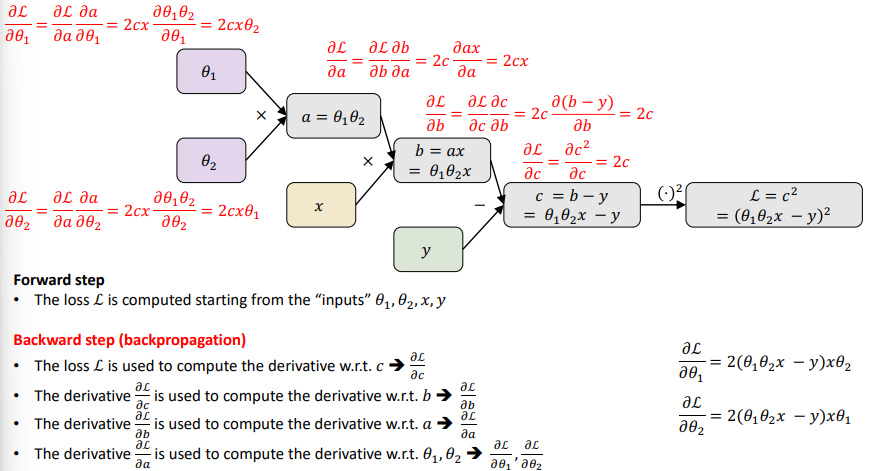
\includegraphics[width=1\linewidth]{content/Parts/images/2026-10-18-17-27-05.png}
  \end{minipage}
  \end{flushleft}

  \section{Loss functions}



  \begin{flushleft}
  \begin{minipage}{0.65\linewidth}

  What loss functin should I use?

  \begin{itemize}
  \item \textbf{Regression}: Mean Squared Error (MSE), Mean Absolute Error (MAE)
  \item \textbf{Binary}: Binary Cross Entropy (BCE), the ground truth is $y = \{0, 1\}$ and the predicted value is $\hat{y} = model(x) \in [0, 1]$


  \item[] \begin{equation*}
    \mathcal{L} = -y\log(\hat{y}) - (1-y)\log(1-\hat{y})
  \end{equation*}

  \item[] Where $y$ is the ground truth, acts as a "selector" of the loss term to be applied.

  \begin{itemize}
  \item[] $y = 1 \to \mathcal{L} = -\log(\hat{y})$
  \item[] $y = 0 \to \mathcal{L} = -\log(1-\hat{y})$
  \end{itemize}
  \end{itemize}

  \begin{itemize}
  \item \textbf{Multi-class classification}:

  \begin{itemize}
  \item  Cross-Entropy
  \item  Generalization to multiple classes of BCE
  \item  $yF = 1$ when ground truth is the ith class, 0 otherwise
  \item  $yF$ plays the same "selector" mechanism as in BCE
\end{itemize}

\end{itemize}

\begin{equation*}
  \mathcal{L} = -\sum_{i} y_i \log(\hat{y}_i)
\end{equation*}


\end{minipage}%
\hfill
\begin{minipage}{0.3\linewidth}
  \centering
  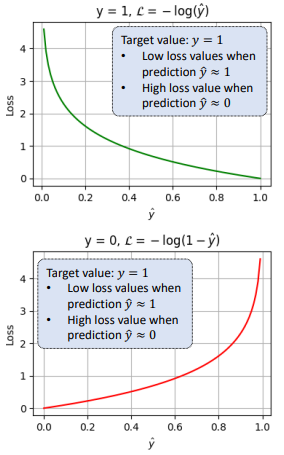
\includegraphics[width=1\linewidth]{content/Parts/images/2026-10-18-17-30-10.png}
\end{minipage}
\end{flushleft}





